A magician skilled in elemental magic, master of destructive energies. Its main Stats are Fire and Water. Its Spells are extremely offensive, which makes it extremely handy in eliminating the opposition, but at the same time aren't very versatile. The list of spells and their description are below, starting at page 64. \pc

\textbf{Representatives}: Black Mage Job (FFI, FFII, FFV, FFX-2, FFXI, FFT, FFTA), Lulu (FFX), Palom of Mysidia (FFIV), Vivi Ornitier (FFIX) \pc

\jobstats[hpa=3x,hpb=4x,hpc=5x,hpd=7x,mpa=3x,mpc=4x,armor=Light,
    weapons=Claws/Gloves \\ Staves \\ Wands]
    
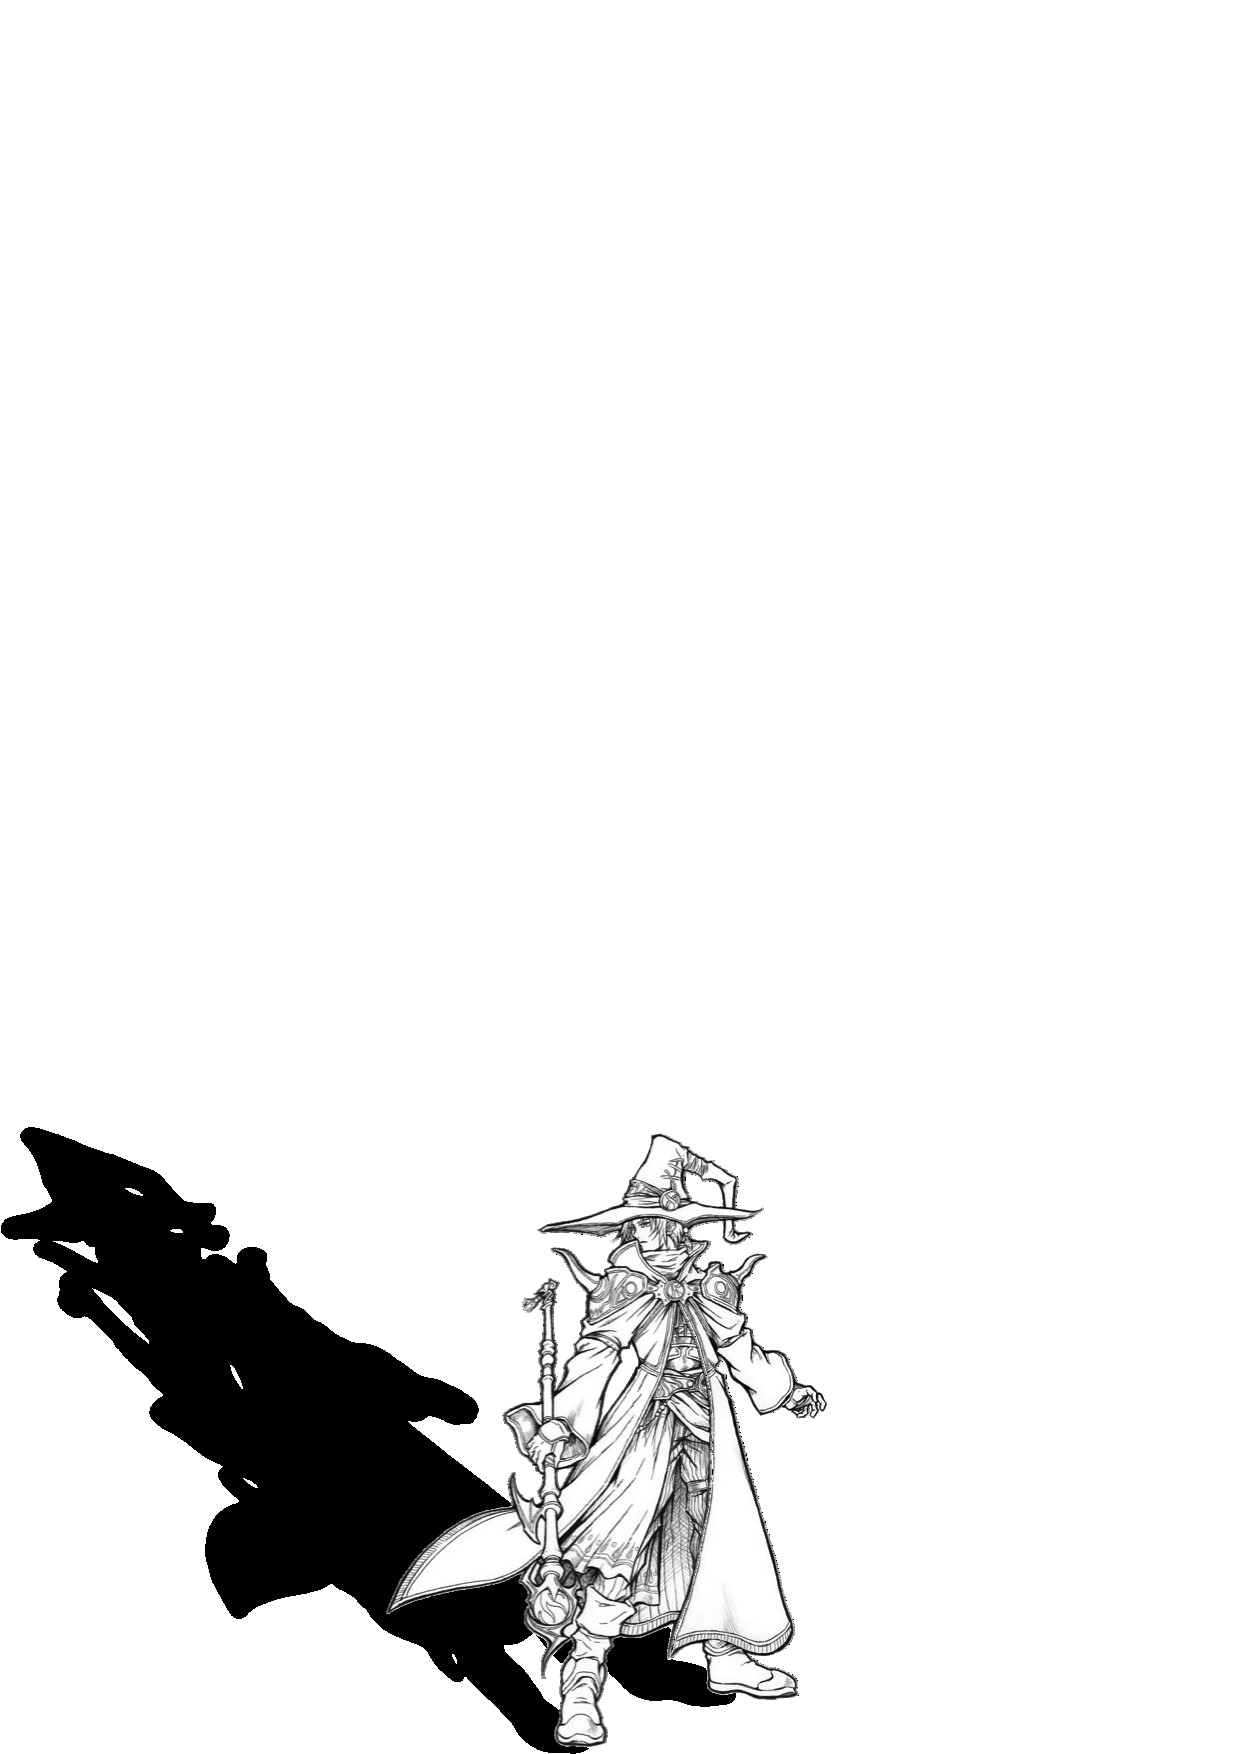
\includegraphics[width=0.3\textwidth,natwidth=829,natheight=627]{"../img/core/revised/blackmage.png"} \par
\begin{ffminipage}
{\centering \textbf{Abilities}\par }

\tability{Arcane Power}: Core ability gained at level 1. You are a black mage, and gain the multipliers and equipment choices above. \pc

\begin{jobspec}
\crystal{level}{12pt} \crystal{fire}{12pt} & %
\tspec{Arcane Mystery: Flare}: Requires Fire level 20 and character level 64. You gain the \tspell{Flare} Spell. \\
\crystal{level}{12pt} \crystal{fire}{12pt} & %
\tspec{Arcane Mystery: Ultima}: Requires Fire level 20 and character level 64. You gain the \tspell{Ultima} Spell. \\
\crystal{level}{12pt} \crystal{fire}{12pt} & %
\tspec{Arcane Mystery: Doomsday}: Requires Fire level 20 and character level 64. You gain the \tspell{Doomsday} Spell. \\
\end{jobspec}
\end{ffminipage}

\begin{ffminipage}
\noindent\tability{Elemental Magic}: Core Ability acquired at level 1. You gain one Elemental Spell group: \tspellgroup{Lightning}, \tspellgroup{Ice}, or \tspellgroup{Fire}. \pc

\begin{jobspec}
\crystal{water}{12pt} & %
\tspec{Elemental Mastery}: Requires Water level 3. You gain one Elemental Spell group. After reaching level 15, gain another Elemental Spell group. \\
\crystal{earth}{12pt} & %
\tspellgroup{Elemental Burst}: Requires Earth level 4. Whenever you use a Spell against a single target, you may deal 25\% of the Spell’s damage to another opponent, chosen randomly, ignoring their MARM. \\
\crystal{fire}{12pt} & %
\tspec{Elemental Shock}: Requires Fire level 5. Whenever you deal damage with an Elemental Spell, increase the value of all targets’ initiative dice by 1, up to a maximum of 10. \\
\end{jobspec}
\end{ffminipage}

\begin{ffminipage}
\noindent\tability{Transmutation}: Core Ability acquired at level 1. You gain one Transmutation Spell group: \tspellgroup{Death}, \tspellgroup{Transform} or \tspellgroup{Poison}. \pc

\begin{jobspec}
\crystal{fire}{12pt} & %
\tspec{Transmutation Mastery}: Requires Fire level 6. You gain one Transmutation Spell group. \\
\crystal{air}{12pt} \crystal{water}{12pt} & %
\tspec{Piercing Arcana}: Requires Air and Water level 5. Your Spells ignore the targets’ status resistance. This has no effect on status immunities. \\
\crystal{earth}{12pt} \crystal{fire}{12pt} & %
\tspec{Magic Resistance}: Requires Earth and Fire level 4. You resist all status effects you are able to inflict with a Transmutation Spell. \\
\end{jobspec}
\end{ffminipage}

\begin{ffminipage}
\noindent\tability{Worldly Magic}: Core Ability acquired at level 15. You gain one Worldly Spell group: \tspellgroup{Water}, \tspellgroup{Earth}, or \tspellgroup{Shadow}. \pc

\begin{jobspec}
\crystal{earth}{12pt} & %
\tspec{Worldly Mastery}: Requires Earth level 8. You gain one Worldly Spell group. \\
\crystal{fire}{12pt} \crystal{water}{12pt} & %
\tspec{Worldly Shock}: Requires Fire level 10 and Water level 7. Your Spells ignore half of targets’ MARM. \\
\crystal{air}{12pt} \crystal{water}{12pt} & %
\tspec{Careful Casting}: Requires Air level 5 and Water level 8. You may, as you cast a Spell, make it a Slow (3) action. Doing so will reduce by 30 its difficulty, to a minimum of zero. All difficulties listed in the Spell are reduced by this effect. \\
\end{jobspec}
\end{ffminipage}

\begin{ffminipage}
\noindent\tability{Magical Expert}: Core Skill acquired at level 30. You gain one Expert Spell group: \tspellgroup{Drain}, \tspellgroup{Hex}, or \tspellgroup{Mage Bane}. \pc

\begin{jobspec}
\crystal{earth}{12pt} \crystal{air}{12pt} \crystal{water}{12pt} & %
\tspec{Multi-Expert}: Requires Earth, Air and Water level 7. You gain one Expert Spell group. \\
\crystal{fire}{12pt} & %
\tspec{Obliterate}: Requires Fire level 12. When you use an Expert Spell, before applying the Spell’s effects, if the target has the \tstatus{Protect}, \tstatus{Shell}, and/or \tstatus{Reflect} statuses they cease to affect him until the end of the round. \\
\crystal{air}{12pt} \crystal{fire}{12pt} & %
\tspec{Favored Element}: Requires Air level 9 and Fire level 10. Choose an element. Your attacks of the chosen element ignore the target’s elemental resistance and deal 50\% damage to immune targets. \\
\end{jobspec}
\end{ffminipage}